\documentclass[12pt,letterpaper]{article}
\usepackage{graphicx,textcomp}
\usepackage{natbib}
\usepackage{setspace}
\usepackage{fullpage}
\usepackage{color}
\usepackage[reqno]{amsmath}
\usepackage{amsthm}
\usepackage{fancyvrb}
\usepackage{amssymb,enumerate}
\usepackage[all]{xy}
\usepackage{endnotes}
\usepackage{lscape}
\newtheorem{com}{Comment}
\usepackage{float}
\usepackage{hyperref}
\newtheorem{lem} {Lemma}
\newtheorem{prop}{Proposition}
\newtheorem{thm}{Theorem}
\newtheorem{defn}{Definition}
\newtheorem{cor}{Corollary}
\newtheorem{obs}{Observation}
\usepackage[compact]{titlesec}
\usepackage{dcolumn}
\usepackage{tikz}
\usetikzlibrary{arrows}
\usepackage{multirow}
\usepackage{xcolor}
\newcolumntype{.}{D{.}{.}{-1}}
\newcolumntype{d}[1]{D{.}{.}{#1}}
\definecolor{light-gray}{gray}{0.65}
\usepackage{url}
\usepackage{listings}
\usepackage{color}

\definecolor{codegreen}{rgb}{0,0.6,0}
\definecolor{codegray}{rgb}{0.5,0.5,0.5}
\definecolor{codepurple}{rgb}{0.58,0,0.82}
\definecolor{backcolour}{rgb}{0.95,0.95,0.92}

\lstdefinestyle{mystyle}{
	backgroundcolor=\color{backcolour},   
	commentstyle=\color{codegreen},
	keywordstyle=\color{magenta},
	numberstyle=\tiny\color{codegray},
	stringstyle=\color{codepurple},
	basicstyle=\footnotesize,
	breakatwhitespace=false,         
	breaklines=true,                 
	captionpos=b,                    
	keepspaces=true,                 
	numbers=left,                    
	numbersep=5pt,                  
	showspaces=false,                
	showstringspaces=false,
	showtabs=false,                  
	tabsize=2
}
\lstset{style=mystyle}
\newcommand{\Sref}[1]{Section~\ref{#1}}
\newtheorem{hyp}{Hypothesis}

\title{Problem Set 2}
\date{Due: February 18, 2024}
\author{Applied Stats II}


\begin{document}
	\maketitle
	\section*{Instructions}
	\begin{itemize}
		\item Please show your work! You may lose points by simply writing in the answer. If the problem requires you to execute commands in \texttt{R}, please include the code you used to get your answers. Please also include the \texttt{.R} file that contains your code. If you are not sure if work needs to be shown for a particular problem, please ask.
		\item Your homework should be submitted electronically on GitHub in \texttt{.pdf} form.
		\item This problem set is due before 23:59 on Sunday February 18, 2024. No late assignments will be accepted.
	%	\item Total available points for this homework is 80.
	\end{itemize}

	
	%	\vspace{.25cm}
	
%\noindent In this problem set, you will run several regressions and create an add variable plot (see the lecture slides) in \texttt{R} using the \texttt{incumbents\_subset.csv} dataset. Include all of your code.

	\vspace{.25cm}
%\section*{Question 1} %(20 points)}
%\vspace{.25cm}
\noindent We're interested in what types of international environmental agreements or policies people support (\href{https://www.pnas.org/content/110/34/13763}{Bechtel and Scheve 2013)}. So, we asked 8,500 individuals whether they support a given policy, and for each participant, we vary the (1) number of countries that participate in the international agreement and (2) sanctions for not following the agreement. \\

\noindent Load in the data labeled \texttt{climateSupport.RData} on GitHub, which contains an observational study of 8,500 observations.

\begin{itemize}
	\item
	Response variable: 
	\begin{itemize}
		\item \texttt{choice}: 1 if the individual agreed with the policy; 0 if the individual did not support the policy
	\end{itemize}
	\item
	Explanatory variables: 
	\begin{itemize}
		\item
		\texttt{countries}: Number of participating countries [20 of 192; 80 of 192; 160 of 192]
		\item
		\texttt{sanctions}: Sanctions for missing emission reduction targets [None, 5\%, 15\%, and 20\% of the monthly household costs given 2\% GDP growth]
		
	\end{itemize}
	
\end{itemize}

\newpage
\noindent Please answer the following questions:

\begin{enumerate}
	\item
	Remember, we are interested in predicting the likelihood of an individual supporting a policy based on the number of countries participating and the possible sanctions for non-compliance.
	\begin{enumerate}
		\item [] Fit an additive model. Provide the summary output, the global null hypothesis, and $p$-value. Please describe the results and provide a conclusion.
      \begin{lstlisting}[language=R] 

# load data
load(url("https://github.com/ASDS-TCD/StatsII_Spring2024/blob/main/datasets/climateSupport.RData?raw=true"))
model <- glm(choice ~ countries + sanctions, data=climateSupport, family=binomial(link="logit"))

#glm model
model <- glm(choice ~ countries + sanctions, data=climateSupport, family=binomial(link="logit"))

# summary of the model
model_summary <- summary(model)

# conduct the ANOVA test
model_anova <- anova(model, test="Chisq")
\end{lstlisting} 
\item model summary output:
\input{model_summary.txt}
\vspace{2cm}
\item ANOVA output 
\input{model_anova.txt}
\vspace{1cm}
\item Result and Conclusion;


glm() function in R is used to fit generalized linear models (GLMs), response variable (choice) is binary; Logistic regression is a type of GLM, the log-odds of the probability of the outcome is modeled as a linear combination of the predictor variables.  The overall conclusion from the model summary output is both the number of participating countries and the structure of sanctions have a significant impact on the support for the policy. The likelihood of supporting policy tends to increase with the number of countries participating increase ( countries. L: coefficient is 0.458, a statistically significant p-value:2e-16) The severity of sanctions increases with the likelihood of an individual supporting the policy decreases.( sanctions.L:  coefficient is -0.276332. the p-value is  statistically significant 3.15e-10)

The ANOVA function with test="Chisq" is used to perform a global null hypothesis test, by comparing two models to see if the full model with the predictors provides a significantly better fit to the data than the null model. The full model includes both the countries and sanctions variables as predictors of the choice outcome. The null model, which is a reduced model that includes only the intercept (no predictors)


Both country and sanctions variables significantly influence the binary choice outcomeWhen the country variable is included in the logistic regression model, it significantly improves the model's ability to predict the binary choice outcome. The reduction of residual deviance by 146.724 points towards a substantial improvement in the fit of the model, The p-value 2.2e-16  provides statistical evidence that this improvement is highly significant; The sanctions variable reduces the residual deviance by 68.426, with a p-value of 9.272e-15, also showing a significant effect but to a lesser degree compared to the country variable.


            %\item
		%How many iterations did it take to find the maximum likelihood estimates?
	\end{enumerate}
	
	\item
	If any of the explanatory variables are significant in this model, then:
	\begin{enumerate}
		\item
		For the policy in which nearly all countries participate [160 of 192], how does increasing sanctions from 5\% to 15\% change the odds that an individual will support the policy? (Interpretation of a coefficient)
%		\item
%		For the policy in which very few countries participate [20 of 192], how does increasing sanctions from 5\% to 15\% change the odds that an individual will support the policy? (Interpretation of a coefficient)

The coefficient for sanctions.L is -0.276. This coefficient means the average change in the log odds of an individual supporting the policy for a one-unit change in sanctions if other variables are constant.	Change from 5\% to 15\% sanctions, let's assume 10\% increase corresponds to a one-unit increase in the sanctions variable. This increase would result in a decrease in the log odds of supporting the policy by the coefficient value multiplied by the change in units (  -0.276 * 1 unit) 

\item
		What is the estimated probability that an individual will support a policy if there are 80 of 192 countries participating with no sanctions? 

  \begin{lstlisting}[language=R] 

intercept <- -0.005665
coef_L <- 0.458452
coef_Q <- -0.009950


# proportional to the number of countries 
L_value <- 80 / 192
Q_value <- L_value^2

log_odds = intercept + (coef_L * L_value) + (coef_Q * Q_value)

# Convert log-odds to probability
probability = exp(log_odds) / (1 + exp(log_odds))
print(probability)
#0.5457787
\end{lstlisting} 
Using the coefficients from the part 1 logistic regression model, sanctions are at 0;  calculation base on L represents a direct scaling of the number of countries, Q represents the square of the linear term 		
\item
		Would the answers to 2a and 2b potentially change if we included the interaction term in this model? Why? 
		\begin{itemize}
			\item Perform a test to see if including an interaction is appropriate.
\begin{lstlisting}[language=R] 

# Fit model with interaction
model_with_interaction <- glm(choice ~ countries * sanctions, family=binomial(link="logit"), data=climateSupport)

# Compare models
anova(model, model_with_interaction, test="Chisq")

\end{lstlisting} 
 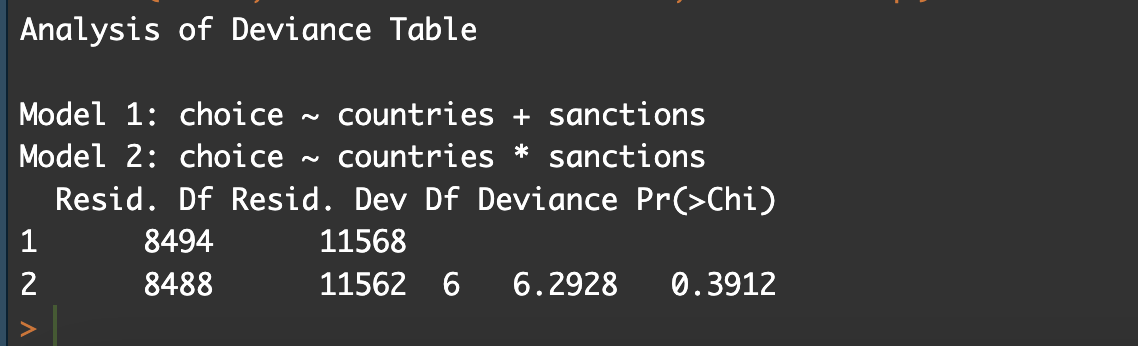
\includegraphics[width=12cm]{Screenshot 2024-02-12 at 20.36.25.png}

 There is no need to include the interaction term in the final model.
 
 Model 1 without interaction term; Model 2 with interaction term. Although Model 1 has a residual deviance of 11568, and Model 2 has a lower residual deviance of 11562, the interaction term may provide a better fit for the data in someway;  The p-value is 0.39. it higher than the significance level of 0.05, which means no statistically significant evidence that the interaction term (between countries and sanctions) improves the model fit for explaining the support for the policy.( response variable: choice)
 
 \end{itemize}
	\end{enumerate}
	\end{enumerate}


\end{document}
